\begin{figure*}
	\centering
	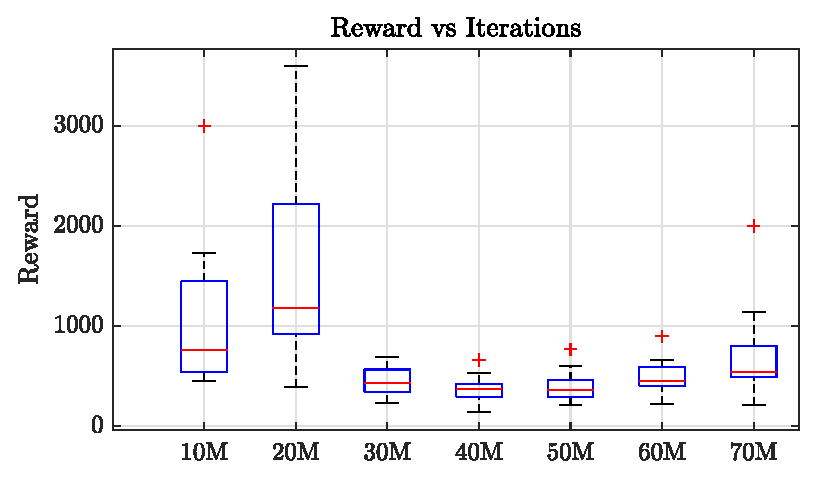
\includegraphics{images/reward_vs_iter.eps}
	\caption{The ability of a trained model to maintain balance while walking is demonstrated. For each model, the box plot considers ten attempts; red line indicates mean value.}
	\label{fig:boxplot}
\end{figure*}

\section{Results}
The bipedal robot has an ankle, knee and hip for each leg (right and left). The dynamic equations of the bipedal robot was computed with MuJoCo software. The reinforcement learning framework,  neural networks and proximal policy optimization algorithm was implemented in Python language using the TensorFlow library, which is an open-source library for artificial intelligence and machine learning. The training of the reinforcement learning agent was carried out on a computed with AMD\textregistered Ryzen 9 94900HS 3.3 GHz processor, 16 GB of RAM, Ubuntu 20.04.3 LTS 64 bits. The Python version 3.8 and the MuJoCo 2.1 were the platforms where the simulations took place.

Figure \ref{fig:boxplot} shows the variation of reward with respect to number of training iterations from $10$ to $70$ millions. In this figure, red line indicates mean value, horizontal lines maximum and minimum values\footnote{visual material of the training of the two-legged robot in \url{https://www.youtube.com/watch?v=gldBp-X0U9k&ab_channel=LucaBorgonovi}}. In this figure, at the beginning, the reward increases with the number of iterations. However, after 20 million iterations the reward decreases dramatically and after 40 million iterations the reward begins to increase. This behavior is related to the way the robot learns to control its body to maximize the reward. On the one hand, up to 20 million iterations the robot only uses one leg (right) to balance its body during the walk. On the other hand, between 20 and 40 million the robot tries to use both legs without knowing how to control the other leg (left). This causes the robot to lose its balance quickly and reduces the amount of reward it will receive. Finally, from 40 million onwards, the robot knows how to control both legs and now only focuses on coordinating the movements of each joint to achieve the walk.




%the reward that model gets with $20$ million is greater than with $10$ million. This is because the model learns to walk better with more training time. However, the reward that model gets with $30$ and $40$ million is less than with $20$ million. This is because model is trying/learning to use both legs instead of just one\footnote{visual material of the training of the two-legged robot in \url{https://www.youtube.com/watch?v=Vt20_SWR2xI&ab_channel=LucaBorgonovi}}.




%To carry out the simulations, the MuJoCo software was used, a simulator for multi-body dynamics with contact. The computational model used to implement the algorithm was a two-dimensional bipedal robot Walker2d-v2, which has 7 joints and two translational movements (horizontal and vertical). During the simulation, the model went through 60 million iterations to assess how gait evolved as the Policy Gradient algorithm was implemented.

%All simulations were carried out on a computer with AMD\textregistered Ryzen 9 94900HS 3.3 GHz processor, 16 GB of RAM, Ubuntu 20.04.3 LTS 64 bits. The Python version 3.8 and the MuJoCo 2.1 were the platforms where the simulations took place.





